% fig_detection_matrix.tex
% TR-25: Stacked bar chart — detection rate by protection element combination
% Shows progression: 87L+87LN → +87LN0 → +TDCS across fault type groups
% Groups: SLG (9 cases), LL (9 cases), 3PH (9 cases)
% Each fault type split by earthing: 3 solid, 3 R-earth, 3 unearthed
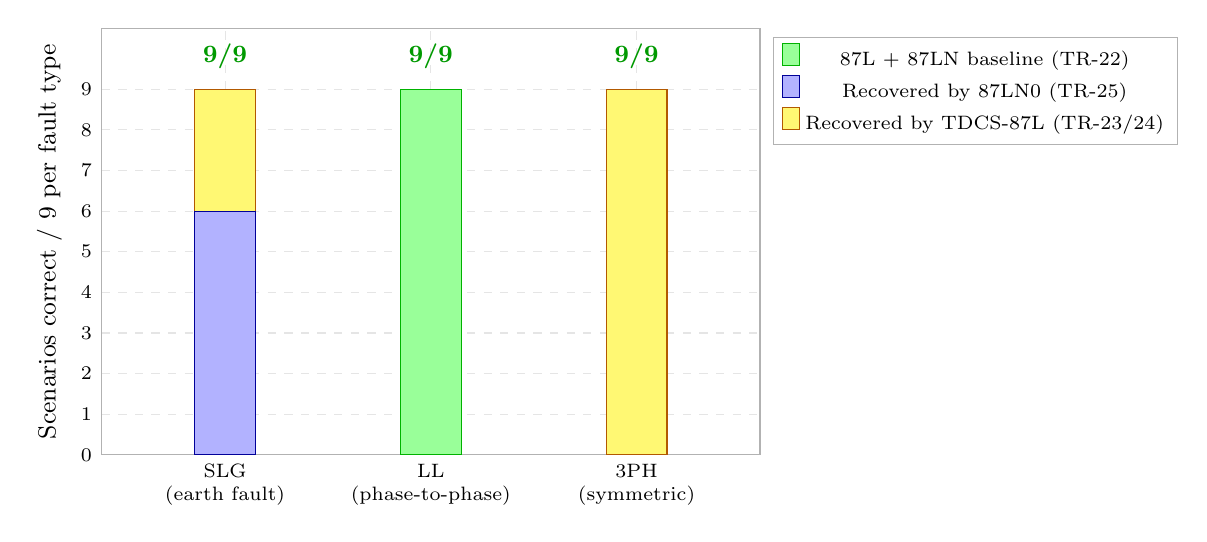
\begin{tikzpicture}
\begin{axis}[
  name         = matax,
  ybar stacked,
  bar width    = 22pt,
  width        = 0.82\textwidth,
  height       = 7.0cm,
  ylabel       = {Scenarios correct / 9 per fault type},
  ylabel style = {font=\small},
  ymin=0, ymax=10.5,
  ytick        = {0,1,2,3,4,5,6,7,8,9},
  yticklabel style={font=\scriptsize},
  xtick        = {1, 2, 3},
  xticklabels  = {SLG\\(earth fault),
                  LL\\(phase-to-phase),
                  3PH\\(symmetric)},
  xticklabel style={font=\scriptsize, align=center},
  enlarge x limits=0.30,
  legend style={at={(1.02,0.98)}, anchor=north west,
                font=\scriptsize, draw=gray!60},
  grid         = major,
  grid style   = {gray!20, dashed},
  tick style   = {draw=none},
  axis line style={gray!60},
]

% Baseline correct by 87L+87LN:
%   SLG: 0/9 (I2≈0, I1<thr)
%   LL:  9/9 (87LN trips, I2=0.10>0.06)
%   3PH: 0/9 (I2=0, I1<thr)
\addplot[fill=green!40, draw=green!70!black]
  coordinates { (1,0) (2,9) (3,0) };
\addlegendentry{87L + 87LN baseline (TR-22)}

% Gained by 87LN0:
%   SLG: solid(3)+R-earth(3) = 6 new trips; unearthed(3) = 0
%   LL:  0 (already covered)
%   3PH: 0 (I0=0, only TDCS can help)
\addplot[fill=blue!30, draw=blue!60!black]
  coordinates { (1,6) (2,0) (3,0) };
\addlegendentry{Recovered by 87LN0 (TR-25)}

% Gained by TDCS:
%   SLG unearthed: 3 (TDCS catches IBR step)
%   LL:  0
%   3PH: 9 (TDCS is the only element that trips)
\addplot[fill=yellow!55, draw=orange!70!black]
  coordinates { (1,3) (2,0) (3,9) };
\addlegendentry{Recovered by TDCS-87L (TR-23/24)}

% Remaining failures: all zero — full coverage achieved (no bar needed)

% Total labels
\node[font=\small\bfseries, green!60!black] at (axis cs:1, 9.8) {9/9};
\node[font=\small\bfseries, green!60!black] at (axis cs:2, 9.8) {9/9};
\node[font=\small\bfseries, green!60!black] at (axis cs:3, 9.8) {9/9};

% Percentage labels per segment
\node[font=\tiny, gray!70!black] at (axis cs:2, 4.5) {9/9};
\node[font=\tiny, blue!70!black] at (axis cs:1, 3.5) {+6};
\node[font=\tiny, orange!70!black] at (axis cs:1, 7.0) {+3};
\node[font=\tiny, orange!70!black] at (axis cs:3, 4.5) {9/9};

\end{axis}
\end{tikzpicture}
